\documentclass[12pt,a4paper]{article}
\usepackage[UTF8]{ctex}
\usepackage{amsmath}
\usepackage{graphicx}
\usepackage{booktabs}
\usepackage{geometry}
\usepackage{siunitx}
\usepackage{pgfplots}
\usepackage{ulem}
\pgfplotsset{compat=1.17}
\geometry{left=2.5cm,right=2.5cm,top=2.5cm,bottom=2.5cm}
\sisetup{per-mode=symbol}

\title{\Huge{\textbf{\uuline{实\ 验\ 报\ 告}}}}
\author{\uline{少年班学院} \quad 姓名: \uline{李大恕} \quad 学号: \uline{PB24000145}}
\date{\today}

\begin{document}
\maketitle

\section{实验题目}
宇宙线$\mu$子平均寿命的测量

\section{实验目的}
\begin{enumerate}
    \item 加深对相对论效应及宇宙线$\mu$子性质的认识。
    \item 掌握宇宙线$\mu$子平均寿命的测量原理。
    \item 学习短时间间隔的一种现代测量方法。
\end{enumerate}

\section{实验原理}
宇宙线$\mu$子主要由高空中产生的$\pi$介子衰变而来。$\mu$子在静止系中的平均寿命约为
\begin{equation}
    \tau_0 \approx \SI{2.197}{\micro\second}.
\end{equation}
若某时刻生成的$\mu$子数为 $N_0$，在时间 $t$ 后尚未衰变的$\mu$子数服从指数衰变规律
\begin{equation}
    N(t)=N_0\mathrm{e}^{-t/\tau_0}.
\end{equation}
因此，若以“到达--衰变”两脉冲之间的时间差作为统计量，则其分布应近似为指数函数。考虑有限分箱宽度后，第 $i$ 个区间 $[t_i,t_{i+1}]$ 内的计数可写成
\begin{equation}
    n_i = \int_{t_i}^{t_{i+1}} \bigl(N_b + A\mathrm{e}^{-t/\tau}\bigr)\,\mathrm{d}t,
\end{equation}
其中 $N_b$ 为背景项，$A$ 为振幅，$\tau$ 为待测平均寿命。

实验装置由闪烁探测器、高压电源、信号处理与数据通讯接口、计算机和分析软件组成。其工作原理是：探测器输出的第一个脉冲作为开始时间，若在预设时间窗内出现第二个脉冲，则记录两者间的时间差；若未出现第二个脉冲，则电路清零重置。通过对大量事件的时间差做频率统计并进行指数拟合，即可得到$\mu$子的平均寿命。

\begin{figure}[htbp]
    \centering
    
\includegraphics[width=0.36\textwidth]{manual_extract/page2_img1.png}
    \caption{$\mu$子产生与衰变过程示意图}
\end{figure}

\begin{figure}[htbp]
    \centering
    
\includegraphics[width=0.82\textwidth]{manual_extract/page4_img1.png}
    \caption{$\mu$子寿命测量装置工作原理图}
\end{figure}

\section{实验过程}
\begin{enumerate}
    \item 将高压电源线、探测器信号线和 USB 通讯线按装置要求连接好，并将探测器工作高压设为 $-\SI{600}{\volt}$。
    \item 观察放大器输出和甄别器输出，调节阈值与延迟，使电路能够稳定输出符合信号。
    \item 在正式测量前进行了阈值扫描，记录阈值与计数的关系。该组点波动相对较大，仅作为选取工作点的参考。
    \item 采集长时长时间差数据和短时长时间差数据，并将原始数据保存为 ASCII 文本文件。
    \item 按 $0\sim20000$、步长 $\SI{1000}{\nano\second}$ 对时间差数据进行频数统计，并用指数函数拟合寿命曲线。
\end{enumerate}

\begin{figure}[htbp]
    \centering
    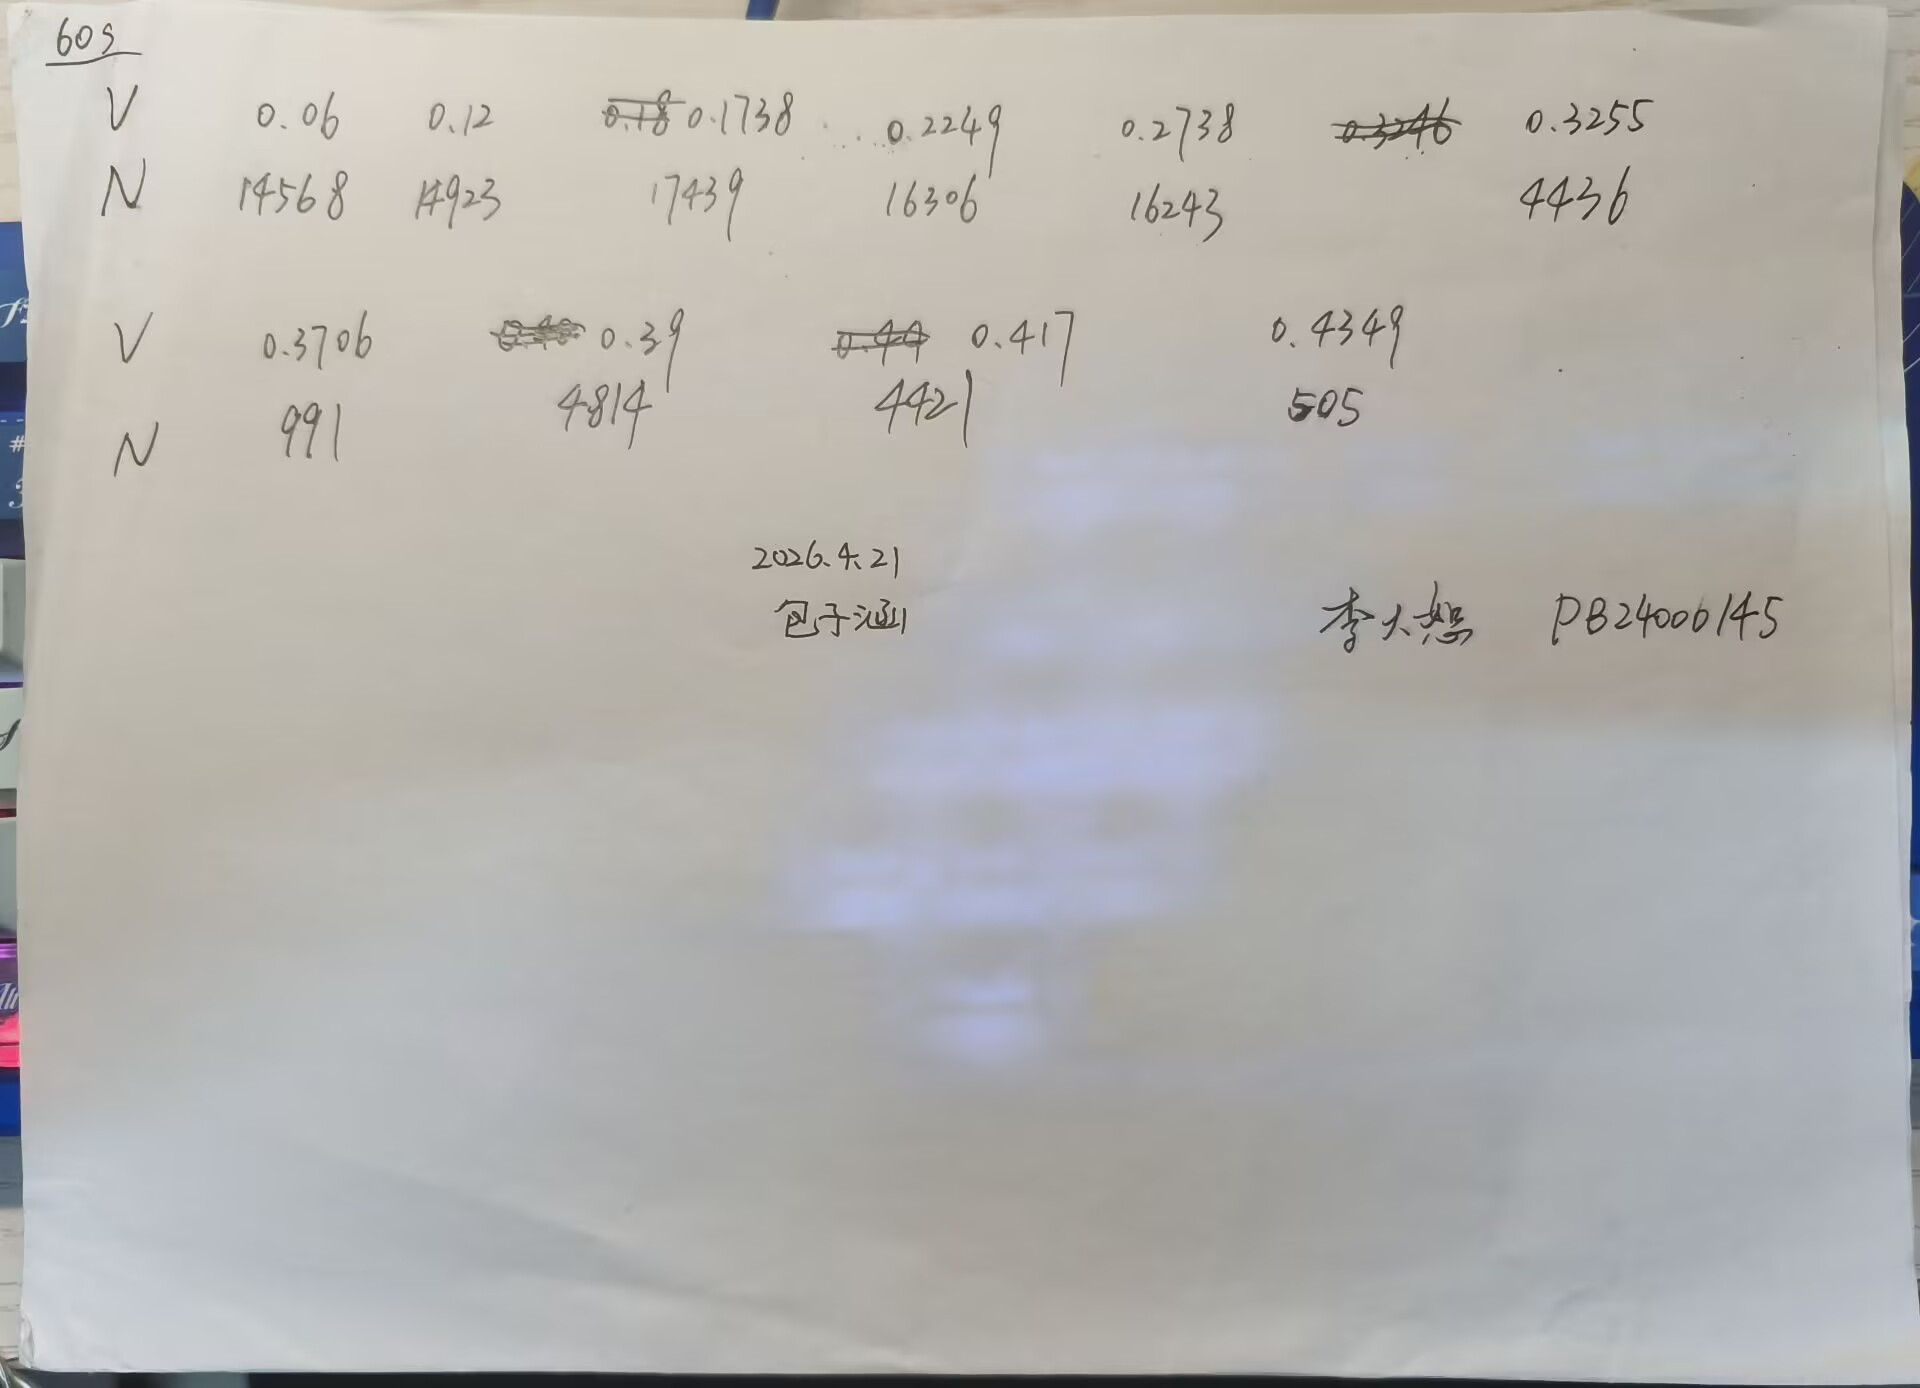
\includegraphics[width=0.9\textwidth]{老师签字的数据.jpg}
    \caption{正式测量前的阈值扫描记录，仅用于辅助确定工作点}
\end{figure}

\section{数据处理与结果}
\subsection{长时长数据的分布与拟合}
将实验室提供的长时长数据按 $\SI{1000}{\nano\second}$ 进行分箱，得到 20 个区间的频数分布。各区间中心点为 500, 1500, \ldots, 19500\,$\si{\nano\second}$。

\begin{figure}[htbp]
\centering
\begin{tikzpicture}
\begin{axis}[
    width=0.86\textwidth,
    height=0.44\textwidth,
    xlabel={时间差 $t$ (\si{\nano\second})},
    ylabel={计数},
    xmin=0, xmax=20000,
    ymin=0, ymax=6000,
    grid=both,
    legend pos=north east,
    mark size=1.5pt
]
\addplot[only marks, blue] coordinates {
    (500,5533) (1500,3682) (2500,2342) (3500,1520) (4500,922)
    (5500,614) (6500,375) (7500,265) (8500,147) (9500,108)
    (10500,86) (11500,61) (12500,47) (13500,25) (14500,27)
    (15500,28) (16500,30) (17500,33) (18500,19) (19500,28)
};
\addplot[red, thick, domain=0:20000, samples=300]
{9.485854 + 6930.303895*exp(-x/2284.238876)};
\legend{分箱频数, 指数拟合}
\end{axis}
\end{tikzpicture}
\caption{长时长数据的时间差分布与指数拟合}
\end{figure}

该数据的拟合函数可写为
\begin{equation}
    N(t)=9.486+6930.304\,\mathrm{e}^{-t/2284.239},
\end{equation}
其中 $t$ 的单位为 $\si{\nano\second}$。由此得到
\begin{equation}
    \tau = \SI{2284.239}{\nano\second} = \SI{2.284\pm0.023}{\micro\second}.
\end{equation}
与理论值 $\SI{2.197}{\micro\second}$ 相比，相对偏差约为 $4.0\%$。

\subsection{短时长数据的分布与拟合}
短时长数据同样按 $\SI{1000}{\nano\second}$ 分箱后作图。由于总事例数较少，高时间区间的计数已经接近统计涨落极限，因此拟合不确定度明显增大。

\begin{figure}[htbp]
\centering
\begin{tikzpicture}
\begin{axis}[
    width=0.86\textwidth,
    height=0.44\textwidth,
    xlabel={时间差 $t$ (\si{\nano\second})},
    ylabel={计数},
    xmin=0, xmax=20000,
    ymin=0, ymax=110,
    grid=both,
    legend pos=north east,
    mark size=1.8pt
]
\addplot[only marks, blue] coordinates {
    (500,101) (1500,53) (2500,34) (3500,19) (4500,15)
    (5500,9) (6500,4) (7500,3) (8500,1) (9500,1)
    (10500,1) (11500,1) (12500,1) (13500,0) (14500,0)
    (15500,2) (16500,0) (17500,0) (18500,0) (19500,0)
};
\addplot[red, thick, domain=0:20000, samples=300]
{1.299728 + 130.334763*exp(-x/1764.504279)};
\legend{分箱频数, 指数拟合}
\end{axis}
\end{tikzpicture}
\caption{短时长数据的时间差分布与指数拟合}
\end{figure}

该数据的拟合函数可写为
\begin{equation}
    N(t)=1.300+130.335\,\mathrm{e}^{-t/1764.504},
\end{equation}
得到
\begin{equation}
    \tau = \SI{1764.504}{\nano\second} = \SI{1.765\pm0.073}{\micro\second}.
\end{equation}
与理论值相比偏差约为 $19.7\%$，说明短时长数据的统计涨落对拟合结果影响较大。

\begin{table}[htbp]
\centering
\caption{两份数据的拟合结果对比}
\begin{tabular}{cccc}
\toprule
数据来源 & 事例数 & 拟合平均寿命 $\tau / \si{\micro\second}$ & 与理论值偏差 \\
\midrule
长时长数据 & 15892 & $2.284\pm0.023$ & 4.0\% \\
短时长数据 & 245 & $1.765\pm0.073$ & 19.7\% \\
理论值 & 无 & 2.197 & 无 \\
\bottomrule
\end{tabular}
\end{table}

\section{思考题}
\begin{enumerate}
    \item \textbf{在地面参考系观测，运动速度为 $0.998c$ 的$\mu$子平均寿命是多少？与实验结果是否矛盾？}\
    不矛盾。地面参考系中，时间膨胀因子为
    \begin{equation}
        \gamma = \frac{1}{\sqrt{1-0.998^2}} \approx 15.8.
    \end{equation}
    因而运动$\mu$子的平均寿命为
    \begin{equation}
        \tau' = \gamma\tau_0 \approx 15.8\times\SI{2.197}{\micro\second} \approx \SI{34.7}{\micro\second}.
    \end{equation}
    这说明高速$\mu$子在地面参考系中可以存活更长时间，并不与实验测得的静止系平均寿命矛盾。

    \item \textbf{该实验是如何保证测量到的两个信号恰是同一$\mu$子的到达与衰变信号？}\
    通过电子学判选实现“先到达、后衰变”的时间关联：第一个符合探测脉冲作为起始信号，若在预设时间窗内出现第二个脉冲，则记录两脉冲间的时间差；若超出时间窗则清零重置。再结合较低的宇宙线计数率和适当阈值，可将偶然符合的比例压低。

    \item \textbf{解释实验测得的$\mu$子衰变寿命曲线具有一定分布的物理原因。}\
    单个$\mu$子的衰变是随机事件，遵从指数衰变统计，因此大量事例的时间差本身就形成指数分布；同时，探测器时间分辨、阈值抖动、背景脉冲和偶然符合都会使曲线在统计上产生离散，特别是在高时间区间计数较少时更明显。

    \item \textbf{比较所测数据与长时长数据结果的差别？实验测量误差可能有哪些来源，如何减少这些误差？}\
    与长时长数据相比，短时长数据的分布更粗糙，长时间区间的计数接近零，指数拟合的参数偏差更大。主要误差来源包括：统计涨落、背景计数、偶然符合、阈值与延迟设置不稳定、电子学死时间以及数据采集时长不足。减少误差的办法是延长采集时间、重新优化阈值和延迟、保持电子学工作点稳定，并尽量减少环境扰动。

    \item \textbf{分析$\mu$氢原子与氢原子在原子半径、结合能方面的差异，并讨论是否可以用$\mu$氘原子实现聚变反应。}\
    由于轨道粒子质量增大，类氢原子的玻尔半径与约化质量成反比，$\mu$原子的轨道半径约为普通氢原子的 $1/186$ 左右；结合能则近似按约化质量成正比，因此$\mu$氢原子的结合能约为普通氢原子的 $186$ 倍，量级约为
    \begin{equation}
        13.6\times 186 \approx \SI{2.5}{\kilo\electronvolt}.
    \end{equation}
    $\mu$氘原子在原理上可以显著缩短核间距，从而提高聚变几率，因此可以实现$\mu$子催化聚变；但实际应用受限于$\mu$子的有限寿命和贴附损失，循环次数不够多时效率不高。
\end{enumerate}

\section{实验结论}
\begin{enumerate}
    \item 按时间差分布对数据进行指数拟合后，长时长数据给出的$\mu$子平均寿命为 $\SI{2.284\pm0.023}{\micro\second}$，与理论值 $\SI{2.197}{\micro\second}$ 一致性较好。
    \item 短时长数据给出的平均寿命为 $\SI{1.765\pm0.073}{\micro\second}$，偏差明显增大，说明事例数不足时统计涨落会显著影响拟合结果。
    \item 正式测量前的阈值扫描数据波动较大，但可用于辅助确定工作点；正式结果主要应以长时长统计为准。
\end{enumerate}

\end{document}